\documentclass[1p]{elsarticle_modified}
%\bibliographystyle{elsarticle-num}

%\usepackage[colorlinks]{hyperref}
%\usepackage{abbrmath_seonhwa} %\Abb, \Ascr, \Acal ,\Abf, \Afrak
\usepackage{amsfonts}
\usepackage{amssymb}
\usepackage{amsmath}
\usepackage{amsthm}
\usepackage{scalefnt}
\usepackage{amsbsy}
\usepackage{kotex}
\usepackage{caption}
\usepackage{subfig}
\usepackage{color}
\usepackage{graphicx}
\usepackage{xcolor} %% white, black, red, green, blue, cyan, magenta, yellow
\usepackage{float}
\usepackage{setspace}
\usepackage{hyperref}

\usepackage{tikz}
\usetikzlibrary{arrows}

\usepackage{multirow}
\usepackage{array} % fixed length table
\usepackage{hhline}

%%%%%%%%%%%%%%%%%%%%%
\makeatletter
\renewcommand*\env@matrix[1][\arraystretch]{%
	\edef\arraystretch{#1}%
	\hskip -\arraycolsep
	\let\@ifnextchar\new@ifnextchar
	\array{*\c@MaxMatrixCols c}}
\makeatother %https://tex.stackexchange.com/questions/14071/how-can-i-increase-the-line-spacing-in-a-matrix
%%%%%%%%%%%%%%%

\usepackage[normalem]{ulem}

\newcommand{\msout}[1]{\ifmmode\text{\sout{\ensuremath{#1}}}\else\sout{#1}\fi}
%SOURCE: \msout is \stkout macro in https://tex.stackexchange.com/questions/20609/strikeout-in-math-mode

\newcommand{\cancel}[1]{
	\ifmmode
	{\color{red}\msout{#1}}
	\else
	{\color{red}\sout{#1}}
	\fi
}

\newcommand{\add}[1]{
	{\color{blue}\uwave{#1}}
}

\newcommand{\replace}[2]{
	\ifmmode
	{\color{red}\msout{#1}}{\color{blue}\uwave{#2}}
	\else
	{\color{red}\sout{#1}}{\color{blue}\uwave{#2}}
	\fi
}

\newcommand{\Sol}{\mathcal{S}} %segment
\newcommand{\D}{D} %diagram
\newcommand{\A}{\mathcal{A}} %arc


%%%%%%%%%%%%%%%%%%%%%%%%%%%%%5 test

\def\sl{\operatorname{\textup{SL}}(2,\Cbb)}
\def\psl{\operatorname{\textup{PSL}}(2,\Cbb)}
\def\quan{\mkern 1mu \triangleright \mkern 1mu}

\theoremstyle{definition}
\newtheorem{thm}{Theorem}[section]
\newtheorem{prop}[thm]{Proposition}
\newtheorem{lem}[thm]{Lemma}
\newtheorem{ques}[thm]{Question}
\newtheorem{cor}[thm]{Corollary}
\newtheorem{defn}[thm]{Definition}
\newtheorem{exam}[thm]{Example}
\newtheorem{rmk}[thm]{Remark}
\newtheorem{alg}[thm]{Algorithm}

\newcommand{\I}{\sqrt{-1}}
\begin{document}

%\begin{frontmatter}
%
%\title{Boundary parabolic representations of knots up to 8 crossings}
%
%%% Group authors per affiliation:
%\author{Yunhi Cho} 
%\address{Department of Mathematics, University of Seoul, Seoul, Korea}
%\ead{yhcho@uos.ac.kr}
%
%
%\author{Seonhwa Kim} %\fnref{s_kim}}
%\address{Center for Geometry and Physics, Institute for Basic Science, Pohang, 37673, Korea}
%\ead{ryeona17@ibs.re.kr}
%
%\author{Hyuk Kim}
%\address{Department of Mathematical Sciences, Seoul National University, Seoul 08826, Korea}
%\ead{hyukkim@snu.ac.kr}
%
%\author{Seokbeom Yoon}
%\address{Department of Mathematical Sciences, Seoul National University, Seoul, 08826,  Korea}
%\ead{sbyoon15@snu.ac.kr}
%
%\begin{abstract}
%We find all boundary parabolic representation of knots up to 8 crossings.
%
%\end{abstract}
%\begin{keyword}
%    \MSC[2010] 57M25 
%\end{keyword}
%
%\end{frontmatter}

%\linenumbers
%\tableofcontents
%
\newcommand\colored[1]{\textcolor{white}{\rule[-0.35ex]{0.8em}{1.4ex}}\kern-0.8em\color{red} #1}%
%\newcommand\colored[1]{\textcolor{white}{ #1}\kern-2.17ex	\textcolor{white}{ #1}\kern-1.81ex	\textcolor{white}{ #1}\kern-2.15ex\color{red}#1	}

{\Large $\underline{12a_{0249}~(K12a_{0249})}$}

\setlength{\tabcolsep}{10pt}
\renewcommand{\arraystretch}{1.6}
\vspace{1cm}\begin{tabular}{m{100pt}>{\centering\arraybackslash}m{274pt}}
\multirow{5}{120pt}{
	\centering
	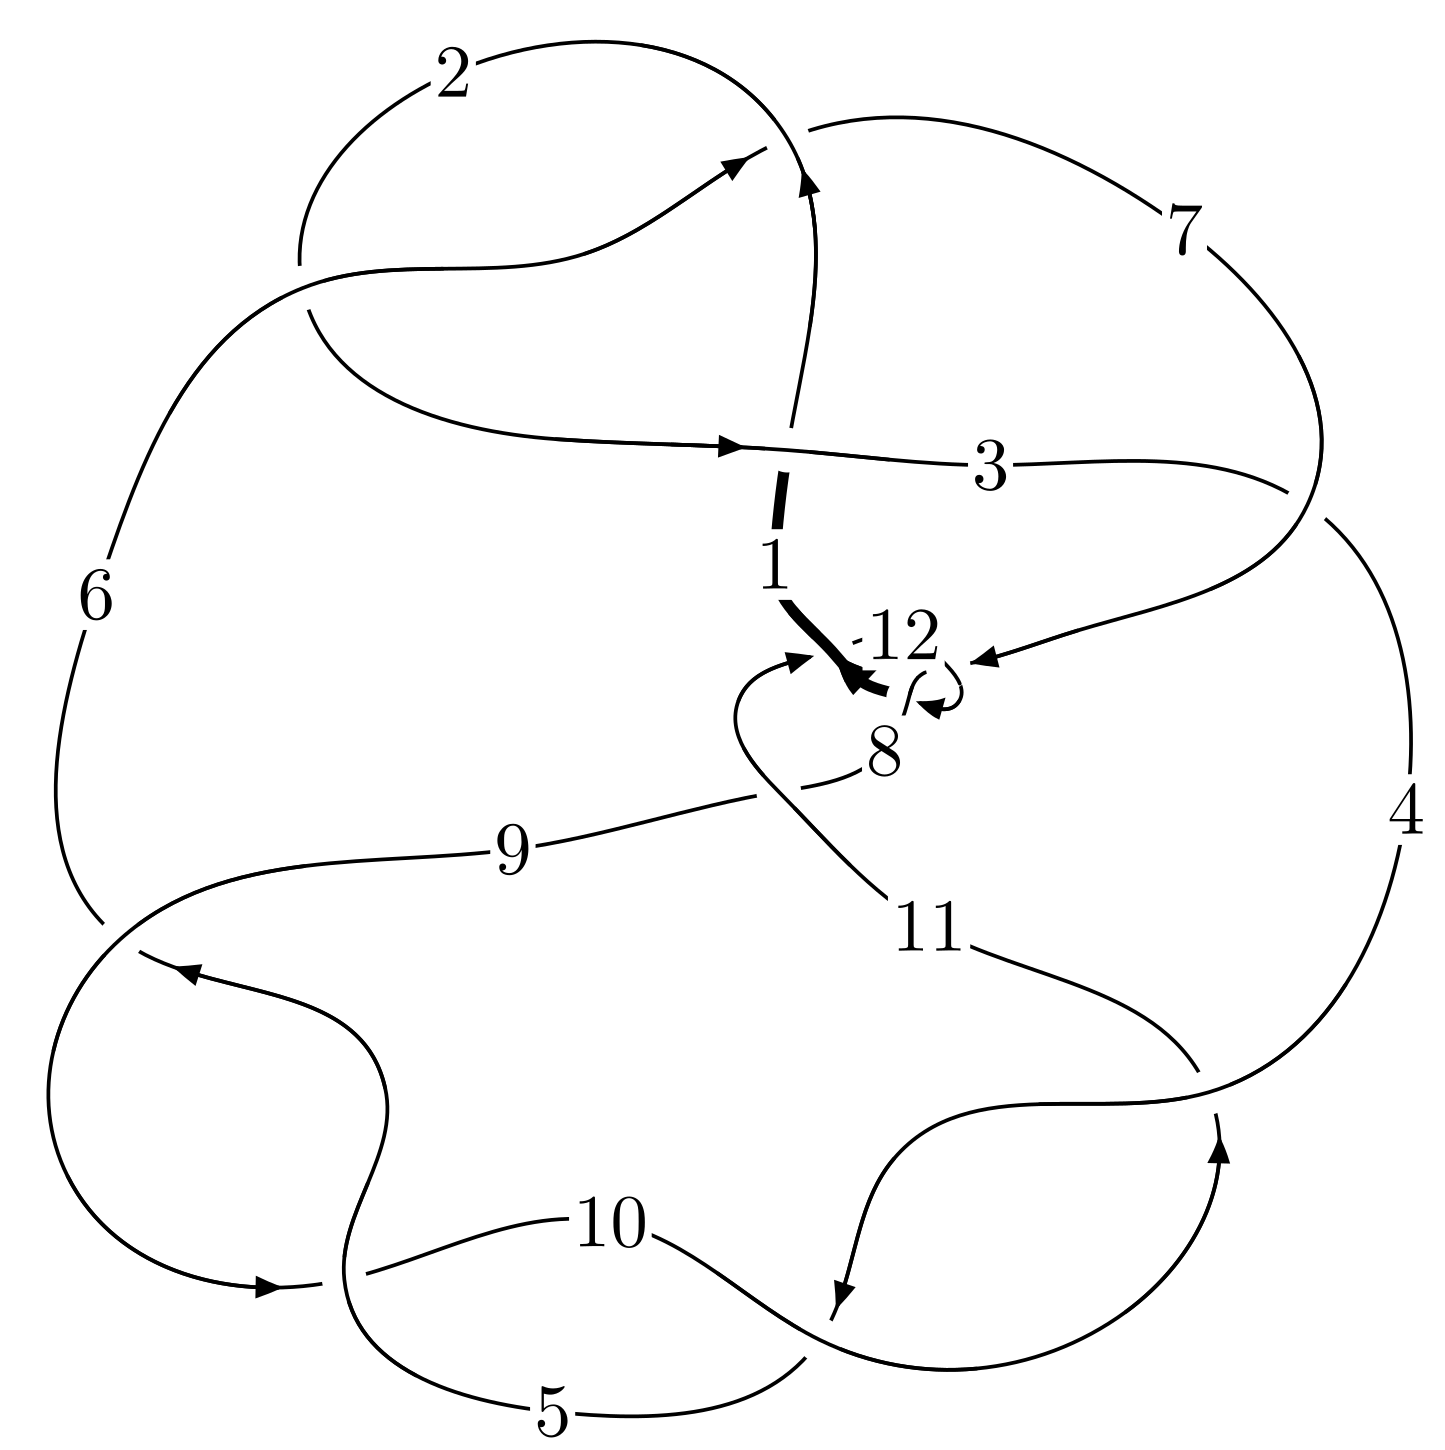
\includegraphics[width=112pt]{../../../GIT/diagram.site/Diagrams/png/1050_12a_0249.png}\\
\ \ \ A knot diagram\footnotemark}&
\allowdisplaybreaks
\textbf{Linearized knot diagam} \\
\cline{2-2}
 &
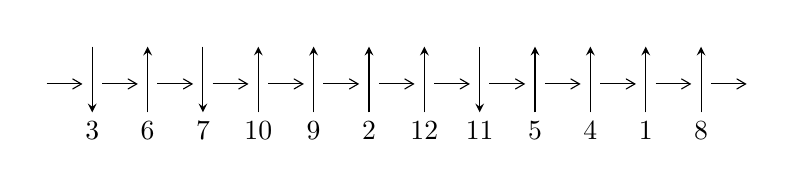
\begin{tikzpicture}[x=20pt, y=17pt]
	% nodes
	\node (C0) at (0, 0) {};
	\node (C1) at (1, 0) {};
	\node (C1U) at (1, +1) {};
	\node (C1D) at (1, -1) {3};

	\node (C2) at (2, 0) {};
	\node (C2U) at (2, +1) {};
	\node (C2D) at (2, -1) {6};

	\node (C3) at (3, 0) {};
	\node (C3U) at (3, +1) {};
	\node (C3D) at (3, -1) {7};

	\node (C4) at (4, 0) {};
	\node (C4U) at (4, +1) {};
	\node (C4D) at (4, -1) {10};

	\node (C5) at (5, 0) {};
	\node (C5U) at (5, +1) {};
	\node (C5D) at (5, -1) {9};

	\node (C6) at (6, 0) {};
	\node (C6U) at (6, +1) {};
	\node (C6D) at (6, -1) {2};

	\node (C7) at (7, 0) {};
	\node (C7U) at (7, +1) {};
	\node (C7D) at (7, -1) {12};

	\node (C8) at (8, 0) {};
	\node (C8U) at (8, +1) {};
	\node (C8D) at (8, -1) {11};

	\node (C9) at (9, 0) {};
	\node (C9U) at (9, +1) {};
	\node (C9D) at (9, -1) {5};

	\node (C10) at (10, 0) {};
	\node (C10U) at (10, +1) {};
	\node (C10D) at (10, -1) {4};

	\node (C11) at (11, 0) {};
	\node (C11U) at (11, +1) {};
	\node (C11D) at (11, -1) {1};

	\node (C12) at (12, 0) {};
	\node (C12U) at (12, +1) {};
	\node (C12D) at (12, -1) {8};
	\node (C13) at (13, 0) {};

	% arrows
	\draw[->,>={angle 60}]
	(C0) edge (C1) (C1) edge (C2) (C2) edge (C3) (C3) edge (C4) (C4) edge (C5) (C5) edge (C6) (C6) edge (C7) (C7) edge (C8) (C8) edge (C9) (C9) edge (C10) (C10) edge (C11) (C11) edge (C12) (C12) edge (C13) ;	\draw[->,>=stealth]
	(C1U) edge (C1D) (C2D) edge (C2U) (C3U) edge (C3D) (C4D) edge (C4U) (C5D) edge (C5U) (C6D) edge (C6U) (C7D) edge (C7U) (C8U) edge (C8D) (C9D) edge (C9U) (C10D) edge (C10U) (C11D) edge (C11U) (C12D) edge (C12U) ;
	\end{tikzpicture} \\
\hhline{~~} \\& 
\textbf{Solving Sequence} \\ \cline{2-2} 
 &
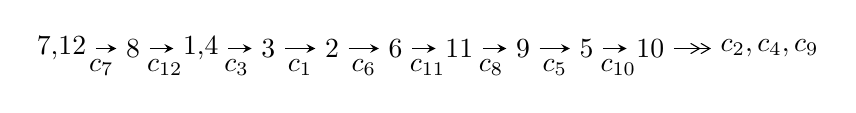
\begin{tikzpicture}[x=23pt, y=7pt]
	% node
	\node (A0) at (-1/8, 0) {7,12};
	\node (A1) at (1, 0) {8};
	\node (A2) at (33/16, 0) {1,4};
	\node (A3) at (25/8, 0) {3};
	\node (A4) at (33/8, 0) {2};
	\node (A5) at (41/8, 0) {6};
	\node (A6) at (49/8, 0) {11};
	\node (A7) at (57/8, 0) {9};
	\node (A8) at (65/8, 0) {5};
	\node (A9) at (73/8, 0) {10};
	\node (C1) at (1/2, -1) {$c_{7}$};
	\node (C2) at (3/2, -1) {$c_{12}$};
	\node (C3) at (21/8, -1) {$c_{3}$};
	\node (C4) at (29/8, -1) {$c_{1}$};
	\node (C5) at (37/8, -1) {$c_{6}$};
	\node (C6) at (45/8, -1) {$c_{11}$};
	\node (C7) at (53/8, -1) {$c_{8}$};
	\node (C8) at (61/8, -1) {$c_{5}$};
	\node (C9) at (69/8, -1) {$c_{10}$};
	\node (A10) at (11, 0) {$c_{2},c_{4},c_{9}$};

	% edge
	\draw[->,>=stealth]	
	(A0) edge (A1) (A1) edge (A2) (A2) edge (A3) (A3) edge (A4) (A4) edge (A5) (A5) edge (A6) (A6) edge (A7) (A7) edge (A8) (A8) edge (A9) ;
	\draw[->>,>={angle 60}]	
	(A9) edge (A10);
\end{tikzpicture} \\ 

\end{tabular} \\

\footnotetext{
The image of knot diagram is generated by the software ``\textbf{Draw programme}" developed by Andrew Bartholomew(\url{http://www.layer8.co.uk/maths/draw/index.htm\#Running-draw}), where we modified some parts for our purpose(\url{https://github.com/CATsTAILs/LinksPainter}).
}\phantom \\ \newline 
\centering \textbf{Ideals for irreducible components\footnotemark of $X_{\text{par}}$} 
 
\begin{align*}
I^u_{1}&=\langle 
-4.50926\times10^{56} u^{80}+1.29640\times10^{57} u^{79}+\cdots+4.18236\times10^{56} b-1.29334\times10^{57},\\
\phantom{I^u_{1}}&\phantom{= \langle  }2.21087\times10^{57} u^{80}-5.78355\times10^{57} u^{79}+\cdots+1.25471\times10^{57} a+6.67332\times10^{57},\;u^{81}-3 u^{80}+\cdots+10 u-3\rangle \\
I^u_{2}&=\langle 
-2 a^3-3 a^2+5 b-10 a-7,\;a^4+2 a^3+7 a^2+6 a+3,\;u-1\rangle \\
I^u_{3}&=\langle 
b+a,\;a^2- a+1,\;u+1\rangle \\
\\
\end{align*}
\raggedright * 3 irreducible components of $\dim_{\mathbb{C}}=0$, with total 87 representations.\\
\footnotetext{All coefficients of polynomials are rational numbers. But the coefficients are sometimes approximated in decimal forms when there is not enough margin.}
\newpage
\renewcommand{\arraystretch}{1}
\centering \section*{I. $I^u_{1}= \langle -4.51\times10^{56} u^{80}+1.30\times10^{57} u^{79}+\cdots+4.18\times10^{56} b-1.29\times10^{57},\;2.21\times10^{57} u^{80}-5.78\times10^{57} u^{79}+\cdots+1.25\times10^{57} a+6.67\times10^{57},\;u^{81}-3 u^{80}+\cdots+10 u-3 \rangle$}
\flushleft \textbf{(i) Arc colorings}\\
\begin{tabular}{m{7pt} m{180pt} m{7pt} m{180pt} }
\flushright $a_{7}=$&$\begin{pmatrix}1\\0\end{pmatrix}$ \\
\flushright $a_{12}=$&$\begin{pmatrix}0\\u\end{pmatrix}$ \\
\flushright $a_{8}=$&$\begin{pmatrix}1\\- u^2\end{pmatrix}$ \\
\flushright $a_{1}=$&$\begin{pmatrix}u\\- u^3+u\end{pmatrix}$ \\
\flushright $a_{4}=$&$\begin{pmatrix}-1.76206 u^{80}+4.60948 u^{79}+\cdots+13.6480 u-5.31862\\1.07816 u^{80}-3.09968 u^{79}+\cdots-4.73997 u+3.09235\end{pmatrix}$ \\
\flushright $a_{3}=$&$\begin{pmatrix}-0.683900 u^{80}+1.50979 u^{79}+\cdots+8.90805 u-2.22626\\1.07816 u^{80}-3.09968 u^{79}+\cdots-4.73997 u+3.09235\end{pmatrix}$ \\
\flushright $a_{2}=$&$\begin{pmatrix}-0.759894 u^{80}+1.19450 u^{79}+\cdots+5.14103 u+1.04489\\1.33087 u^{80}-3.53951 u^{79}+\cdots-12.1484 u+4.61361\end{pmatrix}$ \\
\flushright $a_{6}=$&$\begin{pmatrix}0.488879 u^{80}-0.786987 u^{79}+\cdots-10.5299 u+3.51618\\-0.777576 u^{80}+1.87963 u^{79}+\cdots+9.94260 u-4.09065\end{pmatrix}$ \\
\flushright $a_{11}=$&$\begin{pmatrix}- u^3\\u^5- u^3+u\end{pmatrix}$ \\
\flushright $a_{9}=$&$\begin{pmatrix}u^6- u^4+1\\- u^8+2 u^6-2 u^4\end{pmatrix}$ \\
\flushright $a_{5}=$&$\begin{pmatrix}1.44849 u^{80}-3.72044 u^{79}+\cdots-22.9034 u+8.56114\\-0.149725 u^{80}+0.318455 u^{79}+\cdots+5.31675 u-2.26332\end{pmatrix}$ \\
\flushright $a_{10}=$&$\begin{pmatrix}-0.460801 u^{80}+1.25988 u^{79}+\cdots+4.96189 u+2.03652\\0.269554 u^{80}-0.789293 u^{79}+\cdots-6.79647 u+1.41492\end{pmatrix}$\\&\end{tabular}
\flushleft \textbf{(ii) Obstruction class $= -1$}\\~\\
\flushleft \textbf{(iii) Cusp Shapes $= 3.70974 u^{80}-8.50300 u^{79}+\cdots-53.6156 u+22.8801$}\\~\\
\newpage\renewcommand{\arraystretch}{1}
\flushleft \textbf{(iv) u-Polynomials at the component}\newline \\
\begin{tabular}{m{50pt}|m{274pt}}
Crossings & \hspace{64pt}u-Polynomials at each crossing \\
\hline $$\begin{aligned}c_{1}\end{aligned}$$&$\begin{aligned}
&u^{81}+38 u^{80}+\cdots+43 u-9
\end{aligned}$\\
\hline $$\begin{aligned}c_{2},c_{6}\end{aligned}$$&$\begin{aligned}
&u^{81}-2 u^{80}+\cdots+11 u-3
\end{aligned}$\\
\hline $$\begin{aligned}c_{3}\end{aligned}$$&$\begin{aligned}
&u^{81}+2 u^{80}+\cdots-1897 u-1443
\end{aligned}$\\
\hline $$\begin{aligned}c_{4},c_{5},c_{9}\\c_{10}\end{aligned}$$&$\begin{aligned}
&u^{81}- u^{80}+\cdots+16 u-4
\end{aligned}$\\
\hline $$\begin{aligned}c_{7},c_{12}\end{aligned}$$&$\begin{aligned}
&u^{81}-3 u^{80}+\cdots+10 u-3
\end{aligned}$\\
\hline $$\begin{aligned}c_{8}\end{aligned}$$&$\begin{aligned}
&u^{81}-15 u^{80}+\cdots-2304 u-2304
\end{aligned}$\\
\hline $$\begin{aligned}c_{11}\end{aligned}$$&$\begin{aligned}
&u^{81}-43 u^{80}+\cdots+64 u-9
\end{aligned}$\\
\hline
\end{tabular}\\~\\
\newpage\renewcommand{\arraystretch}{1}
\flushleft \textbf{(v) Riley Polynomials at the component}\newline \\
\begin{tabular}{m{50pt}|m{274pt}}
Crossings & \hspace{64pt}Riley Polynomials at each crossing \\
\hline $$\begin{aligned}c_{1}\end{aligned}$$&$\begin{aligned}
&y^{81}+14 y^{80}+\cdots+6115 y-81
\end{aligned}$\\
\hline $$\begin{aligned}c_{2},c_{6}\end{aligned}$$&$\begin{aligned}
&y^{81}+38 y^{80}+\cdots+43 y-9
\end{aligned}$\\
\hline $$\begin{aligned}c_{3}\end{aligned}$$&$\begin{aligned}
&y^{81}-10 y^{80}+\cdots+88698091 y-2082249
\end{aligned}$\\
\hline $$\begin{aligned}c_{4},c_{5},c_{9}\\c_{10}\end{aligned}$$&$\begin{aligned}
&y^{81}+91 y^{80}+\cdots-320 y-16
\end{aligned}$\\
\hline $$\begin{aligned}c_{7},c_{12}\end{aligned}$$&$\begin{aligned}
&y^{81}-43 y^{80}+\cdots+64 y-9
\end{aligned}$\\
\hline $$\begin{aligned}c_{8}\end{aligned}$$&$\begin{aligned}
&y^{81}+31 y^{80}+\cdots+129466368 y-5308416
\end{aligned}$\\
\hline $$\begin{aligned}c_{11}\end{aligned}$$&$\begin{aligned}
&y^{81}-3 y^{80}+\cdots-116 y-81
\end{aligned}$\\
\hline
\end{tabular}\\~\\
\newpage\flushleft \textbf{(vi) Complex Volumes and Cusp Shapes}
$$\begin{array}{c|c|c}  
\text{Solutions to }I^u_{1}& \I (\text{vol} + \sqrt{-1}CS) & \text{Cusp shape}\\
 \hline 
\begin{aligned}
u &= -0.796748 + 0.593974 I \\
a &= \phantom{-}0.799663 - 0.367206 I \\
b &= \phantom{-}1.062700 + 0.399781 I\end{aligned}
 & -4.32097 - 5.87990 I & \phantom{-0.000000 } 0 \\ \hline\begin{aligned}
u &= -0.796748 - 0.593974 I \\
a &= \phantom{-}0.799663 + 0.367206 I \\
b &= \phantom{-}1.062700 - 0.399781 I\end{aligned}
 & -4.32097 + 5.87990 I & \phantom{-0.000000 } 0 \\ \hline\begin{aligned}
u &= \phantom{-}0.261959 + 0.916099 I \\
a &= -0.120408 + 0.255723 I \\
b &= -1.43910 - 0.79999 I\end{aligned}
 & -8.91041 - 10.05080 I & \phantom{-0.000000 -}0. + 6.04265 I \\ \hline\begin{aligned}
u &= \phantom{-}0.261959 - 0.916099 I \\
a &= -0.120408 - 0.255723 I \\
b &= -1.43910 + 0.79999 I\end{aligned}
 & -8.91041 + 10.05080 I & \phantom{-0.000000 } 0. - 6.04265 I \\ \hline\begin{aligned}
u &= \phantom{-}0.792399 + 0.687957 I \\
a &= -0.157829 + 0.788105 I \\
b &= \phantom{-}1.186470 - 0.176451 I\end{aligned}
 & -9.58949 + 2.60972 I & \phantom{-0.000000 } 0 \\ \hline\begin{aligned}
u &= \phantom{-}0.792399 - 0.687957 I \\
a &= -0.157829 - 0.788105 I \\
b &= \phantom{-}1.186470 + 0.176451 I\end{aligned}
 & -9.58949 - 2.60972 I & \phantom{-0.000000 } 0 \\ \hline\begin{aligned}
u &= \phantom{-}0.384053 + 0.849389 I \\
a &= -0.023158 + 0.734226 I \\
b &= -0.649914 - 0.207937 I\end{aligned}
 & -11.25000 - 2.13855 I & -3.51015 + 0. I\phantom{ +0.000000I} \\ \hline\begin{aligned}
u &= \phantom{-}0.384053 - 0.849389 I \\
a &= -0.023158 - 0.734226 I \\
b &= -0.649914 + 0.207937 I\end{aligned}
 & -11.25000 + 2.13855 I & -3.51015 + 0. I\phantom{ +0.000000I} \\ \hline\begin{aligned}
u &= \phantom{-}0.730334 + 0.780884 I \\
a &= -0.029790 - 1.009360 I \\
b &= -1.145080 - 0.109225 I\end{aligned}
 & -13.24960 - 1.33495 I & \phantom{-0.000000 } 0 \\ \hline\begin{aligned}
u &= \phantom{-}0.730334 - 0.780884 I \\
a &= -0.029790 + 1.009360 I \\
b &= -1.145080 + 0.109225 I\end{aligned}
 & -13.24960 + 1.33495 I & \phantom{-0.000000 } 0\\
 \hline 
 \end{array}$$\newpage$$\begin{array}{c|c|c}  
\text{Solutions to }I^u_{1}& \I (\text{vol} + \sqrt{-1}CS) & \text{Cusp shape}\\
 \hline 
\begin{aligned}
u &= \phantom{-}0.985866 + 0.454997 I \\
a &= \phantom{-}0.07224 - 1.47855 I \\
b &= -0.448117 - 0.062543 I\end{aligned}
 & -0.285086 + 1.117670 I & \phantom{-0.000000 } 0 \\ \hline\begin{aligned}
u &= \phantom{-}0.985866 - 0.454997 I \\
a &= \phantom{-}0.07224 + 1.47855 I \\
b &= -0.448117 + 0.062543 I\end{aligned}
 & -0.285086 - 1.117670 I & \phantom{-0.000000 } 0 \\ \hline\begin{aligned}
u &= -0.750762 + 0.487613 I \\
a &= -0.279558 + 0.636943 I \\
b &= -0.800710 - 0.170169 I\end{aligned}
 & -1.53897 - 2.00741 I & \phantom{-}2.59388 + 4.68854 I \\ \hline\begin{aligned}
u &= -0.750762 - 0.487613 I \\
a &= -0.279558 - 0.636943 I \\
b &= -0.800710 + 0.170169 I\end{aligned}
 & -1.53897 + 2.00741 I & \phantom{-}2.59388 - 4.68854 I \\ \hline\begin{aligned}
u &= \phantom{-}0.261751 + 0.852629 I \\
a &= -0.114458 - 0.339479 I \\
b &= \phantom{-}0.999355 + 0.899928 I\end{aligned}
 & -6.55376 - 4.97042 I & \phantom{-}2.32921 + 2.21243 I \\ \hline\begin{aligned}
u &= \phantom{-}0.261751 - 0.852629 I \\
a &= -0.114458 + 0.339479 I \\
b &= \phantom{-}0.999355 - 0.899928 I\end{aligned}
 & -6.55376 + 4.97042 I & \phantom{-}2.32921 - 2.21243 I \\ \hline\begin{aligned}
u &= -0.663280 + 0.559000 I \\
a &= \phantom{-}0.512229 - 1.231590 I \\
b &= \phantom{-}0.886253 - 0.330986 I\end{aligned}
 & -4.60582 + 1.34073 I & -2.15223 - 0.59245 I \\ \hline\begin{aligned}
u &= -0.663280 - 0.559000 I \\
a &= \phantom{-}0.512229 + 1.231590 I \\
b &= \phantom{-}0.886253 + 0.330986 I\end{aligned}
 & -4.60582 - 1.34073 I & -2.15223 + 0.59245 I \\ \hline\begin{aligned}
u &= -1.042180 + 0.456498 I \\
a &= \phantom{-}1.14852 - 1.99118 I \\
b &= \phantom{-}1.143010 + 0.808091 I\end{aligned}
 & -3.31629 - 4.95466 I & \phantom{-0.000000 } 0 \\ \hline\begin{aligned}
u &= -1.042180 - 0.456498 I \\
a &= \phantom{-}1.14852 + 1.99118 I \\
b &= \phantom{-}1.143010 - 0.808091 I\end{aligned}
 & -3.31629 + 4.95466 I & \phantom{-0.000000 } 0\\
 \hline 
 \end{array}$$\newpage$$\begin{array}{c|c|c}  
\text{Solutions to }I^u_{1}& \I (\text{vol} + \sqrt{-1}CS) & \text{Cusp shape}\\
 \hline 
\begin{aligned}
u &= \phantom{-}1.137170 + 0.079899 I \\
a &= -0.377449 + 0.256412 I \\
b &= \phantom{-}0.459209 - 0.546813 I\end{aligned}
 & \phantom{-}1.12101 + 1.57171 I & \phantom{-0.000000 } 0 \\ \hline\begin{aligned}
u &= \phantom{-}1.137170 - 0.079899 I \\
a &= -0.377449 - 0.256412 I \\
b &= \phantom{-}0.459209 + 0.546813 I\end{aligned}
 & \phantom{-}1.12101 - 1.57171 I & \phantom{-0.000000 } 0 \\ \hline\begin{aligned}
u &= \phantom{-}0.871717 + 0.741478 I \\
a &= -0.136021 - 0.555032 I \\
b &= -1.299770 + 0.292571 I\end{aligned}
 & -12.8356 + 6.9731 I & \phantom{-0.000000 } 0 \\ \hline\begin{aligned}
u &= \phantom{-}0.871717 - 0.741478 I \\
a &= -0.136021 + 0.555032 I \\
b &= -1.299770 - 0.292571 I\end{aligned}
 & -12.8356 - 6.9731 I & \phantom{-0.000000 } 0 \\ \hline\begin{aligned}
u &= -0.241031 + 0.814811 I \\
a &= \phantom{-}0.427694 + 0.255486 I \\
b &= \phantom{-}1.28959 - 0.81268 I\end{aligned}
 & -1.44578 + 7.46970 I & \phantom{-}2.13977 - 7.53803 I \\ \hline\begin{aligned}
u &= -0.241031 - 0.814811 I \\
a &= \phantom{-}0.427694 - 0.255486 I \\
b &= \phantom{-}1.28959 + 0.81268 I\end{aligned}
 & -1.44578 - 7.46970 I & \phantom{-}2.13977 + 7.53803 I \\ \hline\begin{aligned}
u &= -1.092690 + 0.367970 I \\
a &= -1.18215 + 1.63995 I \\
b &= -0.502377 - 0.884483 I\end{aligned}
 & -1.50092 - 0.32300 I & \phantom{-0.000000 } 0 \\ \hline\begin{aligned}
u &= -1.092690 - 0.367970 I \\
a &= -1.18215 - 1.63995 I \\
b &= -0.502377 + 0.884483 I\end{aligned}
 & -1.50092 + 0.32300 I & \phantom{-0.000000 } 0 \\ \hline\begin{aligned}
u &= \phantom{-}1.059850 + 0.475151 I \\
a &= -1.46127 - 1.19278 I \\
b &= \phantom{-}0.98355 + 1.34616 I\end{aligned}
 & -3.49725 + 1.66506 I & \phantom{-0.000000 } 0 \\ \hline\begin{aligned}
u &= \phantom{-}1.059850 - 0.475151 I \\
a &= -1.46127 + 1.19278 I \\
b &= \phantom{-}0.98355 - 1.34616 I\end{aligned}
 & -3.49725 - 1.66506 I & \phantom{-0.000000 } 0\\
 \hline 
 \end{array}$$\newpage$$\begin{array}{c|c|c}  
\text{Solutions to }I^u_{1}& \I (\text{vol} + \sqrt{-1}CS) & \text{Cusp shape}\\
 \hline 
\begin{aligned}
u &= -1.114570 + 0.367085 I \\
a &= \phantom{-}1.40300 - 0.98902 I \\
b &= -1.00338 + 1.14710 I\end{aligned}
 & \phantom{-}3.18584 + 0.47349 I & \phantom{-0.000000 } 0 \\ \hline\begin{aligned}
u &= -1.114570 - 0.367085 I \\
a &= \phantom{-}1.40300 + 0.98902 I \\
b &= -1.00338 - 1.14710 I\end{aligned}
 & \phantom{-}3.18584 - 0.47349 I & \phantom{-0.000000 } 0 \\ \hline\begin{aligned}
u &= -1.079580 + 0.538100 I \\
a &= \phantom{-}0.014477 - 1.406800 I \\
b &= \phantom{-}0.435679 + 0.187011 I\end{aligned}
 & -1.49474 - 4.97988 I & \phantom{-0.000000 } 0 \\ \hline\begin{aligned}
u &= -1.079580 - 0.538100 I \\
a &= \phantom{-}0.014477 + 1.406800 I \\
b &= \phantom{-}0.435679 - 0.187011 I\end{aligned}
 & -1.49474 + 4.97988 I & \phantom{-0.000000 } 0 \\ \hline\begin{aligned}
u &= -1.133020 + 0.423394 I \\
a &= -1.08928 + 1.38321 I \\
b &= \phantom{-}0.372683 - 1.290890 I\end{aligned}
 & \phantom{-}4.43540 - 4.64713 I & \phantom{-0.000000 } 0 \\ \hline\begin{aligned}
u &= -1.133020 - 0.423394 I \\
a &= -1.08928 - 1.38321 I \\
b &= \phantom{-}0.372683 + 1.290890 I\end{aligned}
 & \phantom{-}4.43540 + 4.64713 I & \phantom{-0.000000 } 0 \\ \hline\begin{aligned}
u &= \phantom{-}1.107350 + 0.503133 I \\
a &= \phantom{-}1.06694 + 1.60238 I \\
b &= -0.31789 - 1.48156 I\end{aligned}
 & -2.42474 + 7.07010 I & \phantom{-0.000000 } 0 \\ \hline\begin{aligned}
u &= \phantom{-}1.107350 - 0.503133 I \\
a &= \phantom{-}1.06694 - 1.60238 I \\
b &= -0.31789 + 1.48156 I\end{aligned}
 & -2.42474 - 7.07010 I & \phantom{-0.000000 } 0 \\ \hline\begin{aligned}
u &= -0.709019 + 0.330627 I \\
a &= \phantom{-}0.73488 - 2.03338 I \\
b &= \phantom{-}0.655129 - 0.447564 I\end{aligned}
 & -4.74805 + 1.41615 I & -1.51325 - 0.38964 I \\ \hline\begin{aligned}
u &= -0.709019 - 0.330627 I \\
a &= \phantom{-}0.73488 + 2.03338 I \\
b &= \phantom{-}0.655129 + 0.447564 I\end{aligned}
 & -4.74805 - 1.41615 I & -1.51325 + 0.38964 I\\
 \hline 
 \end{array}$$\newpage$$\begin{array}{c|c|c}  
\text{Solutions to }I^u_{1}& \I (\text{vol} + \sqrt{-1}CS) & \text{Cusp shape}\\
 \hline 
\begin{aligned}
u &= -0.776899 + 0.083863 I \\
a &= \phantom{-}0.30115 + 1.53475 I \\
b &= -0.401413 - 1.092700 I\end{aligned}
 & \phantom{-}1.04110 - 2.31172 I & -0.35449 + 6.19378 I \\ \hline\begin{aligned}
u &= -0.776899 - 0.083863 I \\
a &= \phantom{-}0.30115 - 1.53475 I \\
b &= -0.401413 + 1.092700 I\end{aligned}
 & \phantom{-}1.04110 + 2.31172 I & -0.35449 - 6.19378 I \\ \hline\begin{aligned}
u &= \phantom{-}1.127760 + 0.463136 I \\
a &= \phantom{-}0.67789 + 1.86574 I \\
b &= \phantom{-}0.750120 - 0.981832 I\end{aligned}
 & \phantom{-}4.15856 + 3.15800 I & \phantom{-0.000000 } 0 \\ \hline\begin{aligned}
u &= \phantom{-}1.127760 - 0.463136 I \\
a &= \phantom{-}0.67789 - 1.86574 I \\
b &= \phantom{-}0.750120 + 0.981832 I\end{aligned}
 & \phantom{-}4.15856 - 3.15800 I & \phantom{-0.000000 } 0 \\ \hline\begin{aligned}
u &= -0.376784 + 0.677084 I \\
a &= \phantom{-}0.261702 + 0.830485 I \\
b &= \phantom{-}0.580518 + 0.054748 I\end{aligned}
 & -3.52922 + 0.29348 I & -1.95785 - 1.10416 I \\ \hline\begin{aligned}
u &= -0.376784 - 0.677084 I \\
a &= \phantom{-}0.261702 - 0.830485 I \\
b &= \phantom{-}0.580518 - 0.054748 I\end{aligned}
 & -3.52922 - 0.29348 I & -1.95785 + 1.10416 I \\ \hline\begin{aligned}
u &= \phantom{-}1.176320 + 0.345482 I \\
a &= \phantom{-}1.17168 + 1.12394 I \\
b &= -0.466240 - 1.078130 I\end{aligned}
 & \phantom{-}4.66964 + 0.93016 I & \phantom{-0.000000 } 0 \\ \hline\begin{aligned}
u &= \phantom{-}1.176320 - 0.345482 I \\
a &= \phantom{-}1.17168 - 1.12394 I \\
b &= -0.466240 + 1.078130 I\end{aligned}
 & \phantom{-}4.66964 - 0.93016 I & \phantom{-0.000000 } 0 \\ \hline\begin{aligned}
u &= -0.195107 + 0.743309 I \\
a &= -0.146046 - 0.301093 I \\
b &= -0.751437 + 0.868185 I\end{aligned}
 & \phantom{-}0.66207 + 2.61772 I & \phantom{-}5.49326 - 3.70817 I \\ \hline\begin{aligned}
u &= -0.195107 - 0.743309 I \\
a &= -0.146046 + 0.301093 I \\
b &= -0.751437 - 0.868185 I\end{aligned}
 & \phantom{-}0.66207 - 2.61772 I & \phantom{-}5.49326 + 3.70817 I\\
 \hline 
 \end{array}$$\newpage$$\begin{array}{c|c|c}  
\text{Solutions to }I^u_{1}& \I (\text{vol} + \sqrt{-1}CS) & \text{Cusp shape}\\
 \hline 
\begin{aligned}
u &= \phantom{-}1.124630 + 0.513495 I \\
a &= -0.51301 - 2.18559 I \\
b &= -1.29848 + 0.87661 I\end{aligned}
 & \phantom{-}2.13927 + 8.13542 I & \phantom{-0.000000 } 0 \\ \hline\begin{aligned}
u &= \phantom{-}1.124630 - 0.513495 I \\
a &= -0.51301 + 2.18559 I \\
b &= -1.29848 - 0.87661 I\end{aligned}
 & \phantom{-}2.13927 - 8.13542 I & \phantom{-0.000000 } 0 \\ \hline\begin{aligned}
u &= \phantom{-}0.582369 + 0.482564 I \\
a &= -1.052810 + 0.647545 I \\
b &= -0.762247 + 0.368757 I\end{aligned}
 & -1.47024 + 2.80916 I & \phantom{-}3.39752 - 5.23952 I \\ \hline\begin{aligned}
u &= \phantom{-}0.582369 - 0.482564 I \\
a &= -1.052810 - 0.647545 I \\
b &= -0.762247 - 0.368757 I\end{aligned}
 & -1.47024 - 2.80916 I & \phantom{-}3.39752 + 5.23952 I \\ \hline\begin{aligned}
u &= \phantom{-}1.215240 + 0.294028 I \\
a &= -1.44116 - 0.72897 I \\
b &= \phantom{-}1.09779 + 0.94810 I\end{aligned}
 & \phantom{-}3.09913 - 3.92873 I & \phantom{-0.000000 } 0 \\ \hline\begin{aligned}
u &= \phantom{-}1.215240 - 0.294028 I \\
a &= -1.44116 + 0.72897 I \\
b &= \phantom{-}1.09779 - 0.94810 I\end{aligned}
 & \phantom{-}3.09913 + 3.92873 I & \phantom{-0.000000 } 0 \\ \hline\begin{aligned}
u &= -1.156380 + 0.521926 I \\
a &= -0.40564 + 1.98031 I \\
b &= -0.904152 - 1.051560 I\end{aligned}
 & \phantom{-}3.43804 - 7.35840 I & \phantom{-0.000000 } 0 \\ \hline\begin{aligned}
u &= -1.156380 - 0.521926 I \\
a &= -0.40564 - 1.98031 I \\
b &= -0.904152 + 1.051560 I\end{aligned}
 & \phantom{-}3.43804 + 7.35840 I & \phantom{-0.000000 } 0 \\ \hline\begin{aligned}
u &= -1.242610 + 0.276600 I \\
a &= -1.37285 + 0.87169 I \\
b &= \phantom{-}0.643240 - 0.863021 I\end{aligned}
 & -1.73489 + 1.37096 I & \phantom{-0.000000 } 0 \\ \hline\begin{aligned}
u &= -1.242610 - 0.276600 I \\
a &= -1.37285 - 0.87169 I \\
b &= \phantom{-}0.643240 + 0.863021 I\end{aligned}
 & -1.73489 - 1.37096 I & \phantom{-0.000000 } 0\\
 \hline 
 \end{array}$$\newpage$$\begin{array}{c|c|c}  
\text{Solutions to }I^u_{1}& \I (\text{vol} + \sqrt{-1}CS) & \text{Cusp shape}\\
 \hline 
\begin{aligned}
u &= \phantom{-}1.126650 + 0.608937 I \\
a &= -0.03883 - 1.45490 I \\
b &= -0.487522 + 0.360347 I\end{aligned}
 & -9.02484 + 7.52654 I & \phantom{-0.000000 } 0 \\ \hline\begin{aligned}
u &= \phantom{-}1.126650 - 0.608937 I \\
a &= -0.03883 + 1.45490 I \\
b &= -0.487522 - 0.360347 I\end{aligned}
 & -9.02484 - 7.52654 I & \phantom{-0.000000 } 0 \\ \hline\begin{aligned}
u &= -1.281430 + 0.120938 I \\
a &= \phantom{-}0.689563 - 0.297958 I \\
b &= -0.608778 - 0.197622 I\end{aligned}
 & -5.57684 - 0.74021 I & \phantom{-0.000000 } 0 \\ \hline\begin{aligned}
u &= -1.281430 - 0.120938 I \\
a &= \phantom{-}0.689563 + 0.297958 I \\
b &= -0.608778 + 0.197622 I\end{aligned}
 & -5.57684 + 0.74021 I & \phantom{-0.000000 } 0 \\ \hline\begin{aligned}
u &= -1.168810 + 0.553591 I \\
a &= \phantom{-}0.17533 - 2.20631 I \\
b &= \phantom{-}1.40463 + 0.90541 I\end{aligned}
 & \phantom{-}1.29584 - 12.53390 I & \phantom{-0.000000 } 0 \\ \hline\begin{aligned}
u &= -1.168810 - 0.553591 I \\
a &= \phantom{-}0.17533 + 2.20631 I \\
b &= \phantom{-}1.40463 - 0.90541 I\end{aligned}
 & \phantom{-}1.29584 + 12.53390 I & \phantom{-0.000000 } 0 \\ \hline\begin{aligned}
u &= \phantom{-}0.241156 + 0.647722 I \\
a &= -0.982772 + 0.134931 I \\
b &= -1.079730 - 0.790170 I\end{aligned}
 & -0.36569 - 3.61820 I & \phantom{-}4.43428 + 1.83605 I \\ \hline\begin{aligned}
u &= \phantom{-}0.241156 - 0.647722 I \\
a &= -0.982772 - 0.134931 I \\
b &= -1.079730 + 0.790170 I\end{aligned}
 & -0.36569 + 3.61820 I & \phantom{-}4.43428 - 1.83605 I \\ \hline\begin{aligned}
u &= \phantom{-}1.177720 + 0.571789 I \\
a &= \phantom{-}0.19023 + 2.04474 I \\
b &= \phantom{-}1.03678 - 1.09944 I\end{aligned}
 & -3.81938 + 10.21360 I & \phantom{-0.000000 } 0 \\ \hline\begin{aligned}
u &= \phantom{-}1.177720 - 0.571789 I \\
a &= \phantom{-}0.19023 - 2.04474 I \\
b &= \phantom{-}1.03678 + 1.09944 I\end{aligned}
 & -3.81938 - 10.21360 I & \phantom{-0.000000 } 0\\
 \hline 
 \end{array}$$\newpage$$\begin{array}{c|c|c}  
\text{Solutions to }I^u_{1}& \I (\text{vol} + \sqrt{-1}CS) & \text{Cusp shape}\\
 \hline 
\begin{aligned}
u &= \phantom{-}0.672703\phantom{ +0.000000I} \\
a &= \phantom{-}0.594910\phantom{ +0.000000I} \\
b &= \phantom{-}0.364438\phantom{ +0.000000I}\end{aligned}
 & \phantom{-}0.897326\phantom{ +0.000000I} & \phantom{-}11.7850\phantom{ +0.000000I} \\ \hline\begin{aligned}
u &= -1.308700 + 0.269045 I \\
a &= \phantom{-}1.56537 - 0.53093 I \\
b &= -1.22861 + 0.80896 I\end{aligned}
 & -3.73127 + 6.12115 I & \phantom{-0.000000 } 0 \\ \hline\begin{aligned}
u &= -1.308700 - 0.269045 I \\
a &= \phantom{-}1.56537 + 0.53093 I \\
b &= -1.22861 - 0.80896 I\end{aligned}
 & -3.73127 - 6.12115 I & \phantom{-0.000000 } 0 \\ \hline\begin{aligned}
u &= \phantom{-}1.200190 + 0.591386 I \\
a &= \phantom{-}0.07576 - 2.17871 I \\
b &= -1.49919 + 0.91542 I\end{aligned}
 & -6.0747 + 15.5375 I & \phantom{-0.000000 } 0 \\ \hline\begin{aligned}
u &= \phantom{-}1.200190 - 0.591386 I \\
a &= \phantom{-}0.07576 + 2.17871 I \\
b &= -1.49919 - 0.91542 I\end{aligned}
 & -6.0747 - 15.5375 I & \phantom{-0.000000 } 0 \\ \hline\begin{aligned}
u &= \phantom{-}0.239015 + 0.578600 I \\
a &= -1.11598 - 0.91670 I \\
b &= -0.030929 + 1.252910 I\end{aligned}
 & -4.82432 - 2.73548 I & \phantom{-}2.51992 + 2.65110 I \\ \hline\begin{aligned}
u &= \phantom{-}0.239015 - 0.578600 I \\
a &= -1.11598 + 0.91670 I \\
b &= -0.030929 - 1.252910 I\end{aligned}
 & -4.82432 + 2.73548 I & \phantom{-}2.51992 - 2.65110 I \\ \hline\begin{aligned}
u &= \phantom{-}0.050548 + 0.602586 I \\
a &= \phantom{-}0.600496 - 0.272362 I \\
b &= \phantom{-}0.372734 + 0.903682 I\end{aligned}
 & \phantom{-}1.29638 + 0.88850 I & \phantom{-}7.35607 - 3.92879 I \\ \hline\begin{aligned}
u &= \phantom{-}0.050548 - 0.602586 I \\
a &= \phantom{-}0.600496 + 0.272362 I \\
b &= \phantom{-}0.372734 - 0.903682 I\end{aligned}
 & \phantom{-}1.29638 - 0.88850 I & \phantom{-}7.35607 + 3.92879 I \\ \hline\begin{aligned}
u &= \phantom{-}0.439192 + 0.410436 I \\
a &= \phantom{-}0.52086 + 2.20161 I \\
b &= \phantom{-}0.583399 - 1.272770 I\end{aligned}
 & -5.37037 + 2.23689 I & \phantom{-}0.95673 - 4.12499 I\\
 \hline 
 \end{array}$$\newpage$$\begin{array}{c|c|c}  
\text{Solutions to }I^u_{1}& \I (\text{vol} + \sqrt{-1}CS) & \text{Cusp shape}\\
 \hline 
\begin{aligned}
u &= \phantom{-}0.439192 - 0.410436 I \\
a &= \phantom{-}0.52086 - 2.20161 I \\
b &= \phantom{-}0.583399 + 1.272770 I\end{aligned}
 & -5.37037 - 2.23689 I & \phantom{-}0.95673 + 4.12499 I\\
 \hline 
 \end{array}$$\newpage\newpage\renewcommand{\arraystretch}{1}
\centering \section*{II. $I^u_{2}= \langle -2 a^3-3 a^2+5 b-10 a-7,\;a^4+2 a^3+7 a^2+6 a+3,\;u-1 \rangle$}
\flushleft \textbf{(i) Arc colorings}\\
\begin{tabular}{m{7pt} m{180pt} m{7pt} m{180pt} }
\flushright $a_{7}=$&$\begin{pmatrix}1\\0\end{pmatrix}$ \\
\flushright $a_{12}=$&$\begin{pmatrix}0\\1\end{pmatrix}$ \\
\flushright $a_{8}=$&$\begin{pmatrix}1\\-1\end{pmatrix}$ \\
\flushright $a_{1}=$&$\begin{pmatrix}1\\0\end{pmatrix}$ \\
\flushright $a_{4}=$&$\begin{pmatrix}a\\\frac{2}{5} a^3+\frac{3}{5} a^2+2 a+\frac{7}{5}\end{pmatrix}$ \\
\flushright $a_{3}=$&$\begin{pmatrix}\frac{2}{5} a^3+\frac{3}{5} a^2+3 a+\frac{7}{5}\\\frac{2}{5} a^3+\frac{3}{5} a^2+2 a+\frac{7}{5}\end{pmatrix}$ \\
\flushright $a_{2}=$&$\begin{pmatrix}\frac{1}{5} a^3-\frac{1}{5} a^2+a+\frac{1}{5}\\\frac{2}{5} a^3+\frac{3}{5} a^2+2 a+\frac{2}{5}\end{pmatrix}$ \\
\flushright $a_{6}=$&$\begin{pmatrix}- a\\-\frac{2}{5} a^3-\frac{3}{5} a^2-2 a-\frac{7}{5}\end{pmatrix}$ \\
\flushright $a_{11}=$&$\begin{pmatrix}-1\\1\end{pmatrix}$ \\
\flushright $a_{9}=$&$\begin{pmatrix}1\\-1\end{pmatrix}$ \\
\flushright $a_{5}=$&$\begin{pmatrix}\frac{2}{5} a^3+\frac{3}{5} a^2+2 a+\frac{7}{5}\\-\frac{4}{5} a^3-\frac{6}{5} a^2-5 a-\frac{14}{5}\end{pmatrix}$ \\
\flushright $a_{10}=$&$\begin{pmatrix}\frac{1}{5} a^3-\frac{1}{5} a^2+a+\frac{1}{5}\\-\frac{1}{5} a^3+\frac{1}{5} a^2- a+\frac{9}{5}\end{pmatrix}$\\&\end{tabular}
\flushleft \textbf{(ii) Obstruction class $= 1$}\\~\\
\flushleft \textbf{(iii) Cusp Shapes $= \frac{8}{5} a^3+\frac{12}{5} a^2+8 a+\frac{48}{5}$}\\~\\
\newpage\renewcommand{\arraystretch}{1}
\flushleft \textbf{(iv) u-Polynomials at the component}\newline \\
\begin{tabular}{m{50pt}|m{274pt}}
Crossings & \hspace{64pt}u-Polynomials at each crossing \\
\hline $$\begin{aligned}c_{1},c_{2}\end{aligned}$$&$\begin{aligned}
&(u^2- u+1)^2
\end{aligned}$\\
\hline $$\begin{aligned}c_{3},c_{6}\end{aligned}$$&$\begin{aligned}
&(u^2+u+1)^2
\end{aligned}$\\
\hline $$\begin{aligned}c_{4},c_{5},c_{9}\\c_{10}\end{aligned}$$&$\begin{aligned}
&(u^2+2)^2
\end{aligned}$\\
\hline $$\begin{aligned}c_{7}\end{aligned}$$&$\begin{aligned}
&(u-1)^4
\end{aligned}$\\
\hline $$\begin{aligned}c_{8}\end{aligned}$$&$\begin{aligned}
&u^4
\end{aligned}$\\
\hline $$\begin{aligned}c_{11},c_{12}\end{aligned}$$&$\begin{aligned}
&(u+1)^4
\end{aligned}$\\
\hline
\end{tabular}\\~\\
\newpage\renewcommand{\arraystretch}{1}
\flushleft \textbf{(v) Riley Polynomials at the component}\newline \\
\begin{tabular}{m{50pt}|m{274pt}}
Crossings & \hspace{64pt}Riley Polynomials at each crossing \\
\hline $$\begin{aligned}c_{1},c_{2},c_{3}\\c_{6}\end{aligned}$$&$\begin{aligned}
&(y^2+y+1)^2
\end{aligned}$\\
\hline $$\begin{aligned}c_{4},c_{5},c_{9}\\c_{10}\end{aligned}$$&$\begin{aligned}
&(y+2)^4
\end{aligned}$\\
\hline $$\begin{aligned}c_{7},c_{11},c_{12}\end{aligned}$$&$\begin{aligned}
&(y-1)^4
\end{aligned}$\\
\hline $$\begin{aligned}c_{8}\end{aligned}$$&$\begin{aligned}
&y^4
\end{aligned}$\\
\hline
\end{tabular}\\~\\
\newpage\flushleft \textbf{(vi) Complex Volumes and Cusp Shapes}
$$\begin{array}{c|c|c}  
\text{Solutions to }I^u_{2}& \I (\text{vol} + \sqrt{-1}CS) & \text{Cusp shape}\\
 \hline 
\begin{aligned}
u &= \phantom{-}1.00000\phantom{ +0.000000I} \\
a &= -0.500000 + 0.548188 I \\
b &= \phantom{-}0.500000 + 0.866025 I\end{aligned}
 & -3.28987 - 2.02988 I & \phantom{-}6.00000 + 3.46410 I \\ \hline\begin{aligned}
u &= \phantom{-}1.00000\phantom{ +0.000000I} \\
a &= -0.500000 - 0.548188 I \\
b &= \phantom{-}0.500000 - 0.866025 I\end{aligned}
 & -3.28987 + 2.02988 I & \phantom{-}6.00000 - 3.46410 I \\ \hline\begin{aligned}
u &= \phantom{-}1.00000\phantom{ +0.000000I} \\
a &= -0.50000 + 2.28024 I \\
b &= \phantom{-}0.500000 - 0.866025 I\end{aligned}
 & -3.28987 + 2.02988 I & \phantom{-}6.00000 - 3.46410 I \\ \hline\begin{aligned}
u &= \phantom{-}1.00000\phantom{ +0.000000I} \\
a &= -0.50000 - 2.28024 I \\
b &= \phantom{-}0.500000 + 0.866025 I\end{aligned}
 & -3.28987 - 2.02988 I & \phantom{-}6.00000 + 3.46410 I\\
 \hline 
 \end{array}$$\newpage\newpage\renewcommand{\arraystretch}{1}
\centering \section*{III. $I^u_{3}= \langle b+a,\;a^2- a+1,\;u+1 \rangle$}
\flushleft \textbf{(i) Arc colorings}\\
\begin{tabular}{m{7pt} m{180pt} m{7pt} m{180pt} }
\flushright $a_{7}=$&$\begin{pmatrix}1\\0\end{pmatrix}$ \\
\flushright $a_{12}=$&$\begin{pmatrix}0\\-1\end{pmatrix}$ \\
\flushright $a_{8}=$&$\begin{pmatrix}1\\-1\end{pmatrix}$ \\
\flushright $a_{1}=$&$\begin{pmatrix}-1\\0\end{pmatrix}$ \\
\flushright $a_{4}=$&$\begin{pmatrix}a\\- a\end{pmatrix}$ \\
\flushright $a_{3}=$&$\begin{pmatrix}0\\- a\end{pmatrix}$ \\
\flushright $a_{2}=$&$\begin{pmatrix}-1\\- a+1\end{pmatrix}$ \\
\flushright $a_{6}=$&$\begin{pmatrix}a\\- a\end{pmatrix}$ \\
\flushright $a_{11}=$&$\begin{pmatrix}1\\-1\end{pmatrix}$ \\
\flushright $a_{9}=$&$\begin{pmatrix}1\\-1\end{pmatrix}$ \\
\flushright $a_{5}=$&$\begin{pmatrix}a\\- a\end{pmatrix}$ \\
\flushright $a_{10}=$&$\begin{pmatrix}1\\-1\end{pmatrix}$\\&\end{tabular}
\flushleft \textbf{(ii) Obstruction class $= 1$}\\~\\
\flushleft \textbf{(iii) Cusp Shapes $= 4 a+10$}\\~\\
\newpage\renewcommand{\arraystretch}{1}
\flushleft \textbf{(iv) u-Polynomials at the component}\newline \\
\begin{tabular}{m{50pt}|m{274pt}}
Crossings & \hspace{64pt}u-Polynomials at each crossing \\
\hline $$\begin{aligned}c_{1},c_{3},c_{6}\end{aligned}$$&$\begin{aligned}
&u^2- u+1
\end{aligned}$\\
\hline $$\begin{aligned}c_{2}\end{aligned}$$&$\begin{aligned}
&u^2+u+1
\end{aligned}$\\
\hline $$\begin{aligned}c_{4},c_{5},c_{8}\\c_{9},c_{10}\end{aligned}$$&$\begin{aligned}
&u^2
\end{aligned}$\\
\hline $$\begin{aligned}c_{7},c_{11}\end{aligned}$$&$\begin{aligned}
&(u+1)^2
\end{aligned}$\\
\hline $$\begin{aligned}c_{12}\end{aligned}$$&$\begin{aligned}
&(u-1)^2
\end{aligned}$\\
\hline
\end{tabular}\\~\\
\newpage\renewcommand{\arraystretch}{1}
\flushleft \textbf{(v) Riley Polynomials at the component}\newline \\
\begin{tabular}{m{50pt}|m{274pt}}
Crossings & \hspace{64pt}Riley Polynomials at each crossing \\
\hline $$\begin{aligned}c_{1},c_{2},c_{3}\\c_{6}\end{aligned}$$&$\begin{aligned}
&y^2+y+1
\end{aligned}$\\
\hline $$\begin{aligned}c_{4},c_{5},c_{8}\\c_{9},c_{10}\end{aligned}$$&$\begin{aligned}
&y^2
\end{aligned}$\\
\hline $$\begin{aligned}c_{7},c_{11},c_{12}\end{aligned}$$&$\begin{aligned}
&(y-1)^2
\end{aligned}$\\
\hline
\end{tabular}\\~\\
\newpage\flushleft \textbf{(vi) Complex Volumes and Cusp Shapes}
$$\begin{array}{c|c|c}  
\text{Solutions to }I^u_{3}& \I (\text{vol} + \sqrt{-1}CS) & \text{Cusp shape}\\
 \hline 
\begin{aligned}
u &= -1.00000\phantom{ +0.000000I} \\
a &= \phantom{-}0.500000 + 0.866025 I \\
b &= -0.500000 - 0.866025 I\end{aligned}
 & \phantom{-}1.64493 - 2.02988 I & \phantom{-}12.00000 + 3.46410 I \\ \hline\begin{aligned}
u &= -1.00000\phantom{ +0.000000I} \\
a &= \phantom{-}0.500000 - 0.866025 I \\
b &= -0.500000 + 0.866025 I\end{aligned}
 & \phantom{-}1.64493 + 2.02988 I & \phantom{-}12.00000 - 3.46410 I\\
 \hline 
 \end{array}$$\newpage
\newpage\renewcommand{\arraystretch}{1}
\centering \section*{ IV. u-Polynomials}
\begin{tabular}{m{50pt}|m{274pt}}
Crossings & \hspace{64pt}u-Polynomials at each crossing \\
\hline $$\begin{aligned}c_{1}\end{aligned}$$&$\begin{aligned}
&((u^2- u+1)^3)(u^{81}+38 u^{80}+\cdots+43 u-9)
\end{aligned}$\\
\hline $$\begin{aligned}c_{2}\end{aligned}$$&$\begin{aligned}
&((u^2- u+1)^2)(u^2+u+1)(u^{81}-2 u^{80}+\cdots+11 u-3)
\end{aligned}$\\
\hline $$\begin{aligned}c_{3}\end{aligned}$$&$\begin{aligned}
&(u^2- u+1)(u^2+u+1)^2(u^{81}+2 u^{80}+\cdots-1897 u-1443)
\end{aligned}$\\
\hline $$\begin{aligned}c_{4},c_{5},c_{9}\\c_{10}\end{aligned}$$&$\begin{aligned}
&u^2(u^2+2)^2(u^{81}- u^{80}+\cdots+16 u-4)
\end{aligned}$\\
\hline $$\begin{aligned}c_{6}\end{aligned}$$&$\begin{aligned}
&(u^2- u+1)(u^2+u+1)^2(u^{81}-2 u^{80}+\cdots+11 u-3)
\end{aligned}$\\
\hline $$\begin{aligned}c_{7}\end{aligned}$$&$\begin{aligned}
&((u-1)^4)(u+1)^2(u^{81}-3 u^{80}+\cdots+10 u-3)
\end{aligned}$\\
\hline $$\begin{aligned}c_{8}\end{aligned}$$&$\begin{aligned}
&u^6(u^{81}-15 u^{80}+\cdots-2304 u-2304)
\end{aligned}$\\
\hline $$\begin{aligned}c_{11}\end{aligned}$$&$\begin{aligned}
&((u+1)^6)(u^{81}-43 u^{80}+\cdots+64 u-9)
\end{aligned}$\\
\hline $$\begin{aligned}c_{12}\end{aligned}$$&$\begin{aligned}
&((u-1)^2)(u+1)^4(u^{81}-3 u^{80}+\cdots+10 u-3)
\end{aligned}$\\
\hline
\end{tabular}\newpage\renewcommand{\arraystretch}{1}
\centering \section*{ V. Riley Polynomials}
\begin{tabular}{m{50pt}|m{274pt}}
Crossings & \hspace{64pt}Riley Polynomials at each crossing \\
\hline $$\begin{aligned}c_{1}\end{aligned}$$&$\begin{aligned}
&((y^2+y+1)^3)(y^{81}+14 y^{80}+\cdots+6115 y-81)
\end{aligned}$\\
\hline $$\begin{aligned}c_{2},c_{6}\end{aligned}$$&$\begin{aligned}
&((y^2+y+1)^3)(y^{81}+38 y^{80}+\cdots+43 y-9)
\end{aligned}$\\
\hline $$\begin{aligned}c_{3}\end{aligned}$$&$\begin{aligned}
&((y^2+y+1)^3)(y^{81}-10 y^{80}+\cdots+8.86981\times10^{7} y-2082249)
\end{aligned}$\\
\hline $$\begin{aligned}c_{4},c_{5},c_{9}\\c_{10}\end{aligned}$$&$\begin{aligned}
&y^2(y+2)^4(y^{81}+91 y^{80}+\cdots-320 y-16)
\end{aligned}$\\
\hline $$\begin{aligned}c_{7},c_{12}\end{aligned}$$&$\begin{aligned}
&((y-1)^6)(y^{81}-43 y^{80}+\cdots+64 y-9)
\end{aligned}$\\
\hline $$\begin{aligned}c_{8}\end{aligned}$$&$\begin{aligned}
&y^6(y^{81}+31 y^{80}+\cdots+1.29466\times10^{8} y-5308416)
\end{aligned}$\\
\hline $$\begin{aligned}c_{11}\end{aligned}$$&$\begin{aligned}
&((y-1)^6)(y^{81}-3 y^{80}+\cdots-116 y-81)
\end{aligned}$\\
\hline
\end{tabular}
\vskip 2pc
\end{document}